\documentclass[xcolor=dvipsnames]{beamer}

% ==== 主題 ====
\usetheme{metropolis}
\usefonttheme{professionalfonts}          % 不覆蓋你自訂的字型

% ==== 字型 ====
\usepackage{fontspec}
\usepackage{xeCJK}
\renewcommand{\familydefault}{\rmdefault} % 使用 serif 字體(重點)

% 西文字型:Times New Roman 的開源替代品
\setmainfont{TeX Gyre Termes}[
  Ligatures=TeX,
  BoldFont={* Bold},
  ItalicFont={* Italic}
]

% 中文字型(可改為思源宋體、標楷體等)
\setCJKmainfont{Noto Serif CJK TC}
\setCJKsansfont{Noto Sans CJK TC} % 有需要再用
\setCJKmonofont{Noto Sans Mono CJK TC}

% ==== 數學字型(與正文字體一致)====
\usepackage{unicode-math}
\setmathfont{TeX Gyre Termes Math}

% ==== 套件 ====
\usepackage{amsmath, amssymb}
\usepackage{graphicx}
\usepackage{hyperref}
\usepackage{minted}
\usepackage{fvextra}
\usepackage{xcolor}
\usepackage{booktabs}

% ==== 顏色設定(可選)====
\definecolor{MyBlue}{RGB}{3, 55, 105}
\setbeamercolor{structure}{fg=MyBlue}
\setbeamercolor{block title}{bg=MyBlue,fg=white}
\setbeamercolor{block body}{bg=blue!5}
\setbeamertemplate{section in toc}{%
  \inserttocsectionnumber.~\inserttocsection\par
}

\setminted{
    linenos,                % 行號
    frame=lines,            % 上下框線
    framesep=5pt,           % 程式碼與邊框距離
    numbersep=8pt,          % 行號與程式碼距離
    fontsize=\scriptsize,   % 字體大小
    breaklines,             % 自動換行
    tabsize=4,              % tab 寬度
    rulecolor=\color{black},% 框線顏色
    xleftmargin=1.5em       % 左側縮排
}

\title{Variable Operations}
\author{Tai, Wei Hsuan}
\date{week 2}

\begin{document}
	\begin{frame}
		\titlepage
	\end{frame}


    % course material qrcode
    \begin{frame}
        \frametitle{\href{https://drive.google.com/drive/folders/14Tkn-rddw0k1obeOxkWi00S43M0e9wlW?usp=sharing}{課程簡報}}
        \begin{figure}
            \centering
            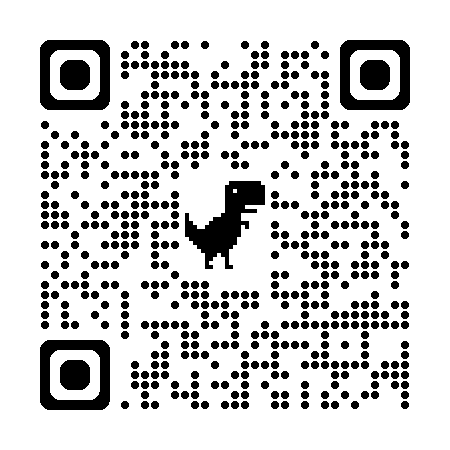
\includegraphics[width=0.7\textwidth]{src/qrcode.png}
        \end{figure}
    \end{frame}

    \begin{frame}
        \frametitle{Outline}
        \tableofcontents
    \end{frame}

    \section{Recap}

    \begin{frame}[fragile]
        \frametitle{Basic Structure of C++ Program}
        \begin{itemize}
            \item Header file.
            \item Namespace.
            \item Main function.
        \end{itemize}
        \begin{minted}{cpp}
            #include <iostream>
            using namespace std;

            int main() {
                cout << "Hello, World!" << endl;
                return 0;
            }
        \end{minted}
    \end{frame}

    \begin{frame}
        \frametitle{Remember!}
        \begin{itemize}
            \item Every statement ends with a semicolon \textbf{(;)}.
            \item Programs always start from the \alert{main()} function.
            \item All functional code needs to be inside a function.
            \item All functions must be enclosed in curly braces \textbf{\{\}}.
        \end{itemize}
    \end{frame}

    \section{Variable Introduction}
    \begin{frame}
        \frametitle{What is Variable?}
        Variables can be thought of as \alert{containers} that hold data which can be changed during program execution.\\
        Data is actually stored in the computer's memory, and variables provide a way to access and manipulate that data.\\
        You can consider variables as \alert{labels} for specific memory locations where data is stored.
    \end{frame}

    \begin{frame}
        \frametitle{Common Data Types}
        \begin{table}[h]
        \centering
        \caption{Common C++ Data Types}
        \begin{tabular}{cll}
        \toprule
        \textbf{Type} & \textbf{Typical Range} & \textbf{Size (bytes)} \\
        \midrule
        \texttt{int}        & $-2^{31}\sim 2^{31}-1$ & 4 \\
        \texttt{long long}  & $-2^{63}\sim 2^{63}-1$ & 8 \\
        \texttt{float}      & $\pm 1.2 \times 10^{-38}\sim 3.4 \times 10^{38}$ & 4 \\
        \texttt{double}     & $\pm 2.3 \times 10^{-308}\sim 1.7 \times 10^{308}$ & 8 \\
        \texttt{char}       & $-2^7\sim 2^7-1$ & 1 \\
        \texttt{bool}     & 0 or 1 & 1 \\
        \bottomrule
        \end{tabular}
        \end{table}        
    \end{frame}

    \section{Variable Operations}
    \begin{frame}
        \frametitle{Operation Types}
        \begin{itemize}
            \item Assignment Operators
            \item Arithmetic Operators
            \item Comparison Operators
            \item Logical Operators
            \item Bitwise Operators
        \end{itemize}
    \end{frame}

    \begin{frame}
        \frametitle{Assignment Operators}
        \begin{table}[h]
        \centering
        \caption{Assignment Operators}
        \begin{tabular}{cll}
        \toprule
        \textbf{Operator} & \textbf{Description} & \textbf{Example} \\
         \midrule
              \texttt{=}   & Assign & \texttt{a = b} \\
                \texttt{+=}  & Add and assign & \texttt{a += b (a = a + b)} \\
                \texttt{-=}  & Subtract and assign & \texttt{a -= b (a = a - b)} \\
                \texttt{*=}  & Multiply and assign & \texttt{a *= b (a = a * b)} \\
                \texttt{/=}  & Divide and assign & \texttt{a /= b (a = a / b)} \\
                \texttt{\%=}  & Modulus and assign & \texttt{a \%= b (a = a \% b)} \\
        \bottomrule
        \end{tabular}
        \end{table}
    \end{frame}
    \begin{frame}[fragile]
        \frametitle{Assignment Operators(Cont.)}
        \begin{minted}{cpp}
            int a=5, b=2;
            a+=b;
            a*=b;
        \end{minted}
    \end{frame}

    \begin{frame}
        \frametitle{Arithmetic Operators}
        \begin{table}[h]
        \centering
        \caption{Arithmetic Operators}
        \begin{tabular}{cll}
        \toprule
        \textbf{Operator} & \textbf{Description} & \textbf{Example} \\
         \midrule
            \texttt{+}  & Addition & a \texttt{+} b \\
            \texttt{-}  & Subtraction & a \texttt{-} b \\
            \texttt{*}  & Multiplication & a \texttt{*} b \\
            \texttt{/}  & Division & a \texttt{/} b \\
            \texttt{\%}  & Modulus (Remainder) & a \texttt{\%} b \\
            \texttt{++} & Increment & \texttt{++}a or a\texttt{++} \\
            \texttt{--} & Decrement & \texttt{--}a or a\texttt{--} \\
        \bottomrule
        \end{tabular}
        \end{table}
    \end{frame}

    \begin{frame}[fragile]
        \frametitle{Arithmetic Operators(Cont.)}
        \begin{minted}{cpp}
            int a=5, b=2;
            cout<<a+b;
            cout<<a%b;
            cout<<++a;
            cout<<b--;
        \end{minted}
        You can also combine assignment and arithmetic operators:
        \begin{minted}{cpp}
            int a=5, b=2;
            int c=a+b, d=b++, e=a/2;//e=2
        \end{minted}
        If the result of division is not an integer, it will be rounded down to the nearest integer.
    \end{frame}
    \begin{frame}
        \frametitle{Comparison Operators}
        \begin{table}[h]
        \centering
        \caption{Comparison Operators}
        This operators always return a boolean value (true or false).
        \begin{tabular}{cll}
        \toprule
        \textbf{Operator} & \textbf{Description} & \textbf{Example} \\
         \midrule
            \texttt{==} & Equal to & a \texttt{==} b \\
            \texttt{!=} & Not equal to & a \texttt{!=} b \\
            \texttt{>}  & Greater than & a \texttt{>} b \\
            \texttt{<}  & Less than & a \texttt{<} b \\
            \texttt{>=} & Greater than or equal to & a \texttt{>=} b \\
            \texttt{<=} & Less than or equal to & a \texttt{<=} b \\
        \bottomrule
        \end{tabular}
        \end{table}
    \end{frame}
    \begin{frame}[fragile]
        \frametitle{Comparison Operators(Cont.)}
        \begin{minted}{cpp}
            int a=5, b=2;
            cout<<(a==b);
            cout<<(a!=b);
            cout<<(a>b);
        \end{minted}
        We will use lots of comparison operators in the condition statements(10/17).
    \end{frame}

    \begin{frame}
        \frametitle{Logical Operators}
        \begin{table}[h]
        \centering
        \caption{Logical Operators}
        This operators always return a boolean value (true or false).
        \begin{tabular}{cll}
        \toprule
        \textbf{Operator} & \textbf{Description} & \textbf{Example} \\
         \midrule
            \texttt{\&\&} & Logical AND & a \texttt{\&\&} b \\
            \texttt{||}  & Logical OR & a \texttt{||} b \\
            \texttt{!}   & Logical NOT & \texttt{!}a \\
        \bottomrule
        \end{tabular}
        \end{table}
        For \texttt{and} and \texttt{or}, exactly you can directly use \texttt{and} and \texttt{or} instead of \texttt{\&\&} and \texttt{||}.
    \end{frame}

    \begin{frame}
        \frametitle{Logical Operators(Cont.)}
        \begin{table}[h]
            \centering
            \begin{tabular}{|c|c||c|c|c|}
                \hline
                \texttt{A} & \texttt{B} & \texttt{!A} & \texttt{A and B} & \texttt{A or B} \\
                \hline
                0 & 0 & 1 & 0 & 0 \\
                0 & 1 & 1 & 0 & 1 \\
                1 & 0 & 0 & 0 & 1 \\
                1 & 1 & 0 & 1 & 1 \\
                \hline
            \end{tabular}
        \end{table}
    \end{frame}

    \begin{frame}[fragile]
        \frametitle{Logical Operators(Cont.)}
        \begin{minted}{cpp}
            int a=5, b=2;
            cout<<((a>b) && (a!=b));
            cout<<((a>b) || (a==b));
            cout<<!(a>b);
        \end{minted}
        Challenge: Determine the result of the following expression:\\
        \texttt{( (1 || 0) \&\& (1 || !1) ) || ( !(0 \&\& 1) \&\& 1 )}
    \end{frame}

    \section{Bitwise Operation}
    \begin{frame}
        \frametitle{Basic concept of Bitwise}
        \begin{itemize}
            \item Data is stored in binary format (0s and 1s).
            \item All the data would be converted into a number and stored in binary format.
            \item In the hardware, high voltage is represented as 1, and low voltage is represented as 0.
            \item Guess it: an empty disk and a full disk, which one is heavier?
            \item All operations in the computer will finally be converted into bitwise operations.
        \end{itemize}
    \end{frame}

    \begin{frame}
        \frametitle{Exponential notation}
        We all learned multiplication in the elementary school. If we want to multiplicate a number by itself several times, we can use exponential notation to represent it.\\
        As the following example:
        $$2^4 = 2 \times 2 \times 2 \times 2 = 16$$
        By definition, $a^b$ means multiplying $a$ by itself $b$ times.\\
    \end{frame}

    \begin{frame}
        \frametitle{Concept of Number Systems}
        A number system represents a value as the sum of powers of its base.
        General form:
        $$
        N = d_k \times b^k + d_{k-1} \times b^{k-1} + \cdots + d_1 \times b^1 + d_0 \times b^0
        $$
        where $b$ is the base, and $d_i$ are the digits.
        Example in base 10 (decimal):
        $$
        345_{10} = 3 \times 10^2 + 4 \times 10^1 + 5 \times 10^0
        $$
        Example in base 2 (binary):
        $$
        1011_2 = 1 \times 2^3 + 0 \times 2^2 + 1 \times 2^1 + 1 \times 2^0 = 11_{10}
        $$
    \end{frame}

    \begin{frame}
        \frametitle{Storage format of Integer}
        For the word, it can be converted into an integer by ASCII code.\\
        We can store integers in binary format, storing binary data in memory is done using bits (0s and 1s). Each bit represents a power of 2, and the combination of bits represents the integer value.\\
        For the aspect of physical, a bit is typically stored using a transistor or a capacitor, where a high voltage represents 1 and a low voltage represents 0.\\
    \end{frame}
    \begin{frame}
        \begin{figure}
            \centering
            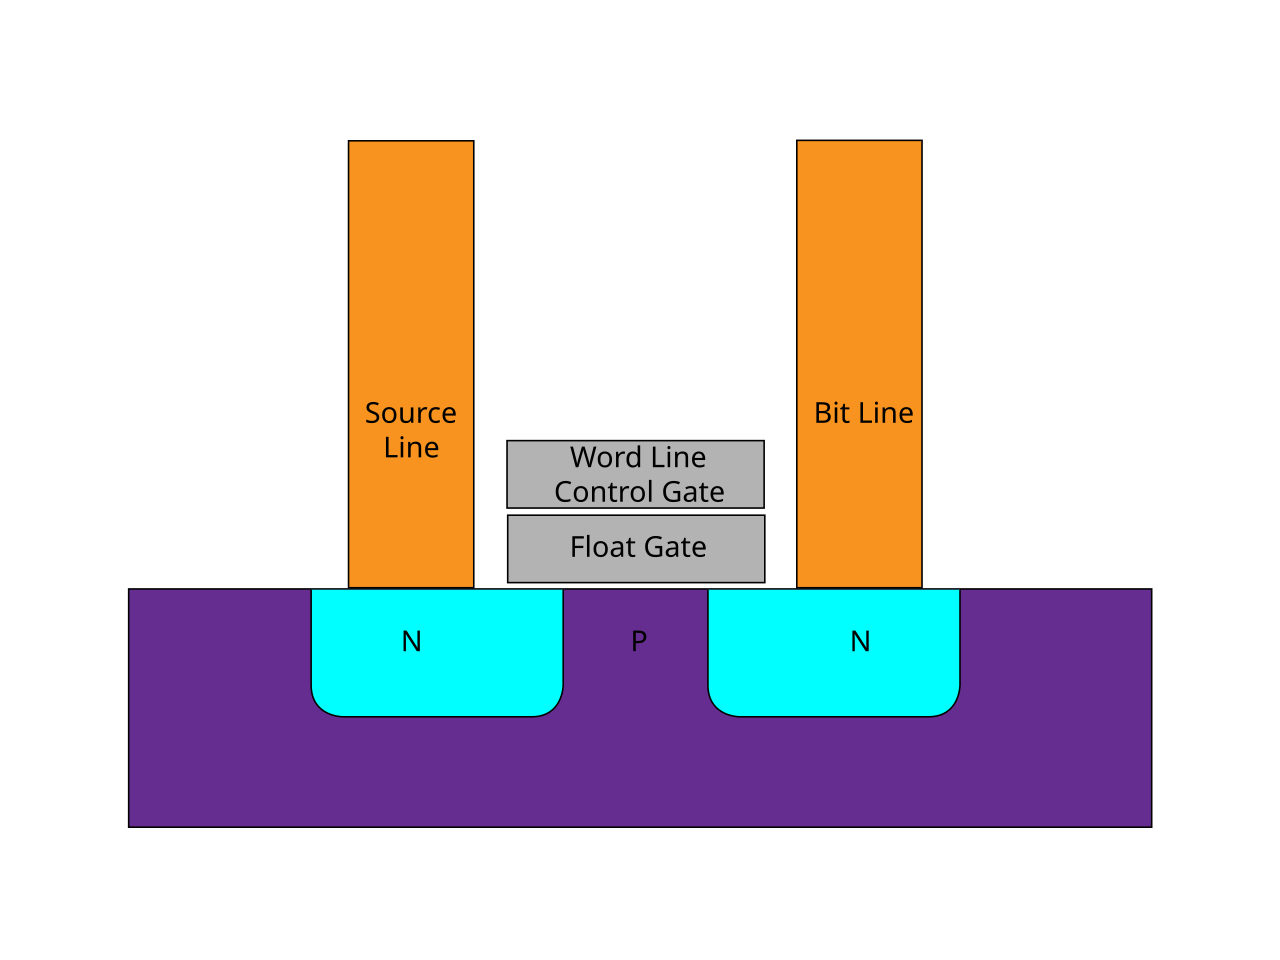
\includegraphics[width=0.8\textwidth]{src/storage.png}
            \caption{Storage principle of Flash memory}
        \end{figure}
        \footnotesize
        Source: Wikipedia
    \end{frame}
    \begin{frame}
        \frametitle{Basic concept of Bitwise operations}
            The operations we learned before are all operations on the entire variables. In this section, we will learn operations on each \alert{bit} of the variable.\\
            Varaibles would be converted into binary format first, and then each bit would be operated according to the rules of bitwise operations.\\
    \end{frame}

    \begin{frame}
        \frametitle{Bitwise Operators}
        \begin{itemize}
            \item AND (\texttt{\&}): Both bits must be 1 to result in 1.
            \item OR (\texttt{\|}): At least one bit must be 1 to result in 1.
            \item XOR (\texttt{ \^ }): Only one bit must be 1 to result in 1.
            \item NOT (\texttt{ \~ }): Inverts the bits (0 becomes 1, and 1 becomes 0).
            \item Left Shift (\texttt{<<}): Shifts bits to the left, filling with 0s on the right.
            \item Right Shift (\texttt{>>}): Shifts bits to the right, filling with 0s on the left (for unsigned types).
        \end{itemize}
        In the following slides, assign \texttt{a=5} and \texttt{b=3} as examples.\\
    \end{frame}

    \begin{frame}
        \frametitle{AND, OR, XOR, NOT}
        First, convert \texttt{a} and \texttt{b} into binary format:
        \begin{align*}
            a &= 5 = 0101_2 \\
            b &= 3 = 0011_2
        \end{align*}
        \begin{table}[h]
            \centering
            \begin{tabular}{c || c c || c | c | c | c}
                \toprule
                Bit Position & \texttt{a} & \texttt{b} & \texttt{and} & \texttt{or} & \texttt{xor} & \texttt{not a} \\
                \midrule
                3 & 0 & 0 & 0 & 0 & 0 & 1 \\
                2 & 1 & 0 & 0 & 1 & 1 & 0 \\
                1 & 0 & 1 & 0 & 1 & 1 & 1 \\
                0 & 1 & 1 & 1 & 1 & 0 & 0 \\
                \bottomrule
            \end{tabular}
        \end{table}
    \end{frame}
    \begin{frame}[fragile]
        \frametitle{AND, OR, XOR, NOT(Cont.)}
        \begin{minted}{cpp}
            int a=5, b=3;
            cout<<(a & b);   // 1
            cout<<(a | b);   // 7
            cout<<(a ^ b);   // 6
            cout<<(~a);    // -6
        \end{minted}
        Note: The result of NOT operation is negative because of the two's complement representation of negative numbers in binary.
    \end{frame}

    \begin{frame}
        \frametitle{Shift Operators}
        The shift operators are actually shift the bits to left or right.\\
        Consider $a=5=0101\_2$:
        \begin{align*}
            a << 1 &= 1010_2 = 10  \\
            a >> 1 &= 0010_2 = 2
        \end{align*}
        Each bit shifted to the left is equivalent to multiplying the number by 2, and each bit shifted to the right is equivalent to dividing the number by 2 (discarding any remainder).
    \end{frame}

    \section{Practice}
    \begin{frame}
        \frametitle{Practice}
        \begin{itemize}
            \item Basic: a002, d827, d485
            \item Advanced: d060, a799, d068, d073, d460
            \item Weird: f987
        \end{itemize}
    \end{frame}
\end{document}